\documentclass[11pt, oneside]{article}   	% use "amsart" instead of "article" for AMSLaTeX format
\usepackage{geometry}                		% See geometry.pdf to learn the layout options. There are lots.
\geometry{letterpaper}                   		% ... or a4paper or a5paper or ... 
%\geometry{landscape}                		% Activate for for rotated page geometry
%\usepackage[parfill]{parskip}    		% Activate to begin paragraphs with an empty line rather than an indent
\usepackage{graphicx}				% Use pdf, png, jpg, or eps� with pdflatex; use eps in DVI mode
								% TeX will automatically convert eps --> pdf in pdflatex		
\usepackage{amssymb}
\usepackage{amsmath}
\usepackage{parskip}
\usepackage{color}
\usepackage{listings}

\title{Using SSH for remote login}
%\author{The Author}
%\section{}
% \subsection*{R code}
\date{}							% Activate to display a given date or no date

\graphicspath{{/Users/telliott_admin/Dropbox/Tex/png/}}

% \begin{center} 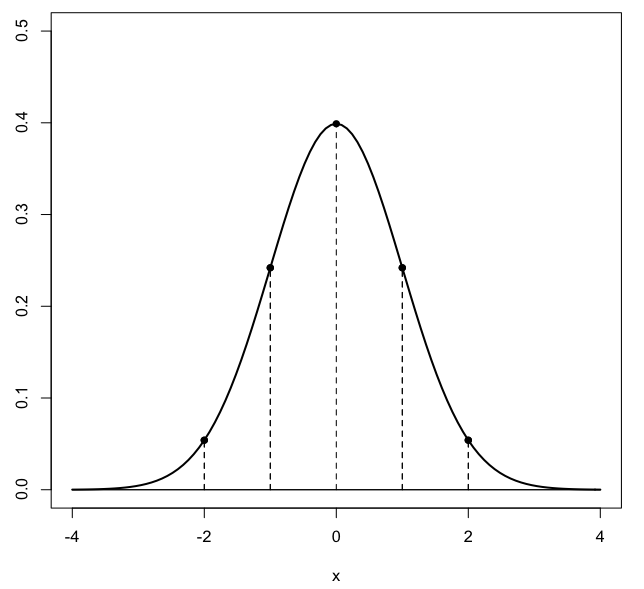
\includegraphics [scale=0.4] {gauss3.png} \end{center}
% \begin{bmatrix} a  &  b \\ c  &  d \end{bmatrix}
% \bigg |_

\begin{document}
\maketitle
\large
%\noindent

Various utilities for ssh are in /usr/bin
\begin{verbatim}
$ ls /usr/bin/ssh*
/usr/bin/ssh          /usr/bin/ssh-keygen
/usr/bin/ssh-add      /usr/bin/ssh-keyscan
/usr/bin/ssh-agent
\end{verbatim}

ssh-keygen with the -l flag:

\begin{verbatim}
     -l      Show fingerprint of specified public
             key file.  Private RSA1 keys are also
             supported.  For RSA and DSA keys
             ssh-keygen tries to find the matching
             public key file and prints its finger-
             print.  If combined with -v, an ASCII
             art representation of the key is sup-
             plied with the fingerprint.
\end{verbatim}

So, for example

\begin{verbatim}
$ ssh-keygen -l -f /private/etc/ssh_host_rsa_key.pub
2048 66:9d:5e:28:32:60:65:ec:99:77:09:87:73:f4:4b:c7   (RSA)
$
\end{verbatim}

gives the fingerprint and (with the -v flag), the ASCII art representation of the public key that my machine uses when it acts as a file server for remote connections.  Try to connect:

\begin{verbatim}
$ ssh telliott_admin@127.0.0.1
ssh: connect to host 127.0.0.1 port 22: Connection refused
\end{verbatim}

Turn on remote login in System Prefs (and turn off WiFi if you're as paranoid as I am), and then from a new Terminal window

\begin{verbatim}
$ ssh telliott_admin@127.0.0.1
The authenticity of host '127.0.0.1 (127.0.0.1)' can't be established.
RSA key fingerprint is 66:9d:5e:28:32:60:65:ec:99:77:09:87:73:f4:4b:c7.
\end{verbatim}

Since the fingerprint matches what we got by \emph{direct inspection} of the host's RSA public key, we're good.

\begin{verbatim}
$ ssh telliott_admin@127.0.0.1
The authenticity of host '127.0.0.1 (127.0.0.1)' can't be established.
RSA key fingerprint is 66:9d:5e:28:32:60:65:ec:99:77:09:87:73:f4:4b:c7.
Are you sure you want to continue connecting (yes/no)? y
Please type 'yes' or 'no': yes 
Warning: Permanently added '127.0.0.1' (RSA) to the list of known hosts.
Password:
Last login: Sat Oct 26 09:24:37 2013
$
\end{verbatim}

What's happened is that the client, my account (which is the same one I'm trying to login to, for convenience), has added 127.0.0.1 (local host) to the list of known hosts.  Note that \emph{You should never see this message again}.  If that happens, it would suggest that a "man in the middle" is trying to impersonate the server.  

Take a look 

\begin{verbatim}
$ cat ~/.ssh/known_hosts 
localhost ssh-rsa AAAAB3NzaC1yc2EAAAADAQABAAABAQDO4Kjzv0/I+TPblXy6jH..
127.0.0.1 ssh-rsa AAAAB3NzaC1yc2EAAAADAQABAAABAQDO4Kjzv0/I+TPblXy6jH..
$
\end{verbatim}

I've truncated the keys here.

I'm not sure where the localhost entry came from, if it's a dup generated at the same time, or it pre-existed.  In any case, what we have in this file is the public key from the server, as seen by

\begin{verbatim}
$ cat /private/etc/ssh_host_rsa_key.pub
ssh-rsa AAAAB3NzaC1yc2EAAAADAQABAAABAQDO4Kjzv0/I+TPblXy6jH..
\end{verbatim}

Alternatively

\begin{verbatim}
$ ssh-keygen -l -f ~/.ssh/known_hosts 
2048 66:9d:5e:28:32:60:65:ec:99:77:09:87:73:f4:4b:c7 localhost (RSA)
2048 66:9d:5e:28:32:60:65:ec:99:77:09:87:73:f4:4b:c7 127.0.0.1 (RSA)
\end{verbatim}

So ssh-keygen does what one would hope for, even when there are multiple keys in the file.  Now, if we're really on a separate box, this is more impressive:

\begin{verbatim}
say I sure love being inside this fancy computer
\end{verbatim}

To logout just do:

\begin{verbatim}
exit
\end{verbatim}

The next step is to use RSA keys to authenticate the login, rather than my account password.  To generate a key pair, do

\begin{verbatim}
ssh-keygen -b 1024 -t dsa
\end{verbatim}

The -b flag specifies the number of bits in the key.  The default is 2048 bits, except that (as the manual says) DSA keys must be exactly 1024 bits, and we're asking for -t dsa.

\begin{verbatim}
$ ssh-keygen -b 1024 -t dsa
Generating public/private dsa key pair.
Enter file in which to save the key (/Users/telliott_admin/.ssh/id_dsa): 
Enter passphrase (empty for no passphrase): 
Enter same passphrase again: 
Your identification has been saved in /Users/telliott_admin/.ssh/id_dsa.
Your public key has been saved in /Users/telliott_admin/.ssh/id_dsa.pub.
The key fingerprint is:
b8:40:02:6f:68:e0:80:0b:74:5e:17:85:b0:9f:ac:2d 
telliott_admin@Toms-MacBook-Air.local
The key's randomart image is:
+--[ DSA 1024]----+
|*. . o.o+.       |
|*+o . o.         |
|o++...           |
|o. o  o..        |
|    . .+S        |
|     .o.         |
|     E..         |
|      .          |
|                 |
+-----------------+
$
\end{verbatim}

So, if I look in .ssh

\begin{verbatim}
$ ssh-keygen -l -f ~/.ssh/id_dsa.pub
1024 b8:40:02:6f:68:e0:80:0b:74:5e:17:85:b0:9f:ac:2d  
telliott_admin@Toms-MacBook-Air.local (DSA)
$ ls ~/.ssh
id_dsa		id_dsa.pub	known_hosts
$
\end{verbatim}

The fingerprints match.  Remember your passphrase!  

The next step is to copy my public key to the server.  First, logon using the password method, then

\begin{verbatim}
$ ssh telliott_admin@127.0.0.1
Password:
Last login: Sat Oct 26 09:38:08 2013 from localhost
$ scp ~/.ssh/id_dsa.pub telliott_admin@127.0.0.1:~/.ssh/authorized_keys
Password:
id_dsa.pub                                100\%  627     0.6KB/s   00:00
\end{verbatim}


In this last part, the "password" is my "passphrase".

\begin{verbatim}
$ exit
logout
Connection to 127.0.0.1 closed.
$ ssh telliott_admin@127.0.0.1
\end{verbatim}

\begin{center} 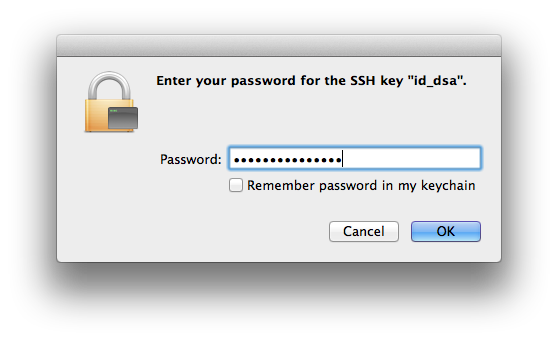
\includegraphics [scale=0.4] {ssh.png} \end{center}

\begin{verbatim}
Saving password to keychain failed
Identity added: /Users/telliott_admin/.ssh/id_dsa 
(/Users/telliott_admin/.ssh/id_dsa)
Last login: Sat Oct 26 09:49:15 2013 from localhost
$
\end{verbatim}

It's quite straightforward now.  I just do ssh from Terminal, and a window pops up asking for my password for my public key, and the rest just works.  Of course, from my client machine, I don't actually need this password to examine the file:

\begin{verbatim}
$ cat ~/.ssh/id_dsa.pub
ssh-dss AAAAB3NzaC1kc3MAAACBAMnTdjVKoV4eKMlWYNOeBOJ10uFGoBTdQdTPZ0+guXo3McUSO..
oQ== telliott_admin@Toms-MacBook-Air.local
$ ssh-keygen -l -f ~/.ssh/id_dsa.pub
1024 b8:40:02:6f:68:e0:80:0b:74:5e:17:85:b0:9f:ac:2d  
telliott_admin@Toms-MacBook-Air.local (DSA)
$
\end{verbatim}

That's the basic approach to setting up remote login via ssh on OS X.

\end{document}  